\documentclass[a4paper,11pt, hidelinks]{article}
\usepackage[left=2cm, top=3cm, text={17cm,24cm}]{geometry}
\usepackage{times}
\usepackage[czech]{babel}
\usepackage[utf8]{inputenc}
\usepackage{multirow}
\usepackage{subcaption}
\usepackage{hyperref}
\usepackage{graphics}
\usepackage{graphicx}
\usepackage{picture}
\usepackage{pdflscape}
\usepackage{lipsum}
\usepackage[linesnumbered,ruled,onelanguage,czech,commentsnumbered,longend]{algorithm2e}

\begin{document}
\SetNlSkip{-1em}
\setlength{\unitlength}{1cm}

\begin{titlepage}
    \begin{center}
        {\Huge \textsc{Vysoké učení technické v Brně}\\}
        {\huge \textsc{Fakulta informačních technologií}\\}
        \vspace{\stretch{0.382}}
        {\LARGE Typografie a publikování\,--\,3. projekt}\\[0.4em]
        {\Huge Tabulky a obrázky \\}
        \vspace{\stretch{0.618}}
    \end{center}

    {\Large \today \hfill David Svaty (xsvaty01)}
\end{titlepage}

\label{page:1}

\section{Úvodní strana}
\label{sec:1}
Název práce umístněte do zlatého řezu a nezapomeňte uvést \uv{dnešní} (today) datum a vaše jméno a příjmení.

\section{Tabulky}
\label{sec:2}
Pro sázení tabulek můžeme použít prostředí \texttt{tabbing} nebo prostředí \texttt{tabular}.

\subsection{Prostředí \texttt{tabbing}}
Při použití \texttt{tabbing} vypadá tabulka následovně:
\begin{tabbing}
    \textbf{Ovoce} \hspace{16mm} \= \textbf{Cena} \hspace{4mm} \= \textbf{Množství} \\
    Jablka \> 25,90 \> 3 kg \\
    Hrušky \> 27,40 \> 2,5 kg \\
    Vodní melouny \> 35,- \> 1 kus \\
\end{tabbing}
Toto prostředí se dá také použít pro sázení algoritmů, ovšem vhodnější je použít prostředí \texttt{alogorithm} nebo \texttt{algorithm2e} (viz sekce \ref*{sec:3}).

\subsection{Prostředí \texttt{tabular}}
Další možností, jak vytvořit tabulku je prostředí \texttt{tabular}. Tabulky pak budou vypadat takto\footnote[1]{Kdyby byl problém s \texttt{cline}, zkuste se podívat třeba sem: http://www.abclinuxu.cz/tex/poradna/show/325037.\\[6em]}: %TODO: zmen

\begin{table}[h]
\catcode`\-=12
\centering
\begin{tabular}{|c|c|c|}
    \hline
    \multirow{2}{*}{\textbf{Měna}} & \multicolumn{2}{|c|}{\textbf{Cena}} \\
    \cline{2-3} %TODO: fix
     & \textbf{nákup} & \textbf{prodej} \\
    \hline
    EUR & 22,705 & 25,242 \\
    GBP & 25,931 & 28,828 \\
    USD & 21,347 & 23,732 \\
    \hline
\end{tabular}
\caption{Tabulka kurzů k dnešnímu dni}
\label{tab:1}
\end{table}

\begin{table}[h]
\catcode`\-=12
\centering
\begin{subtable}[h]{0.085\textwidth}
    \centering
    \begin{tabular}{|c|c|}
        \hline
        \textit{A} & $\neg$\textit{A} \\
        \hline
        \textbf{P} & N \\
        \hline
        \textbf{O} & O \\
        \hline
        \textbf{X} & X \\
        \hline
        \textbf{N} & P \\
        \hline
    \end{tabular}
\end{subtable}
\;
\begin{subtable}{0.235\textwidth}
    \centering
    \begin{tabular}{|c|c|c|c|c|c|}
        \hline
        \multicolumn{2}{|c|}{\multirow{2}{*}{\textit{A} $\land$ \textit{B}}} & \multicolumn{4}{|c|}{\textit{B}} \\
        \cline{3-6}
        \multicolumn{2}{|c|}{} &\textbf{P} & \textbf{O} & \textbf{X} & \textbf{N} \\
        \hline
        \multirow{4}{*}{\textit{A}} & \textbf{P} & P & O & X & N \\
        \cline{2-6}
        & \textbf{O} & O & O & N & N \\
        \cline{2-6}
        & \textbf{X} & X & N & X & N \\
        \cline{2-6}
        & \textbf{N} & N & N & N & N \\
        \hline 
    \end{tabular}
\end{subtable}
\;
\begin{subtable}{0.235\textwidth}
    \centering
    \begin{tabular}{|c|c|c|c|c|c|}
        \hline
        \multicolumn{2}{|c|}{\multirow{2}{*}{\textit{A} $\lor$ \textit{B}}} & \multicolumn{4}{|c|}{\textit{B}} \\
        \cline{3-6}
        \multicolumn{2}{|c|}{} &\textbf{P} & \textbf{O} & \textbf{X} & \textbf{N} \\
        \hline
        \multirow{4}{*}{\textit{A}} & \textbf{P} & P & P & P & P \\
        \cline{2-6}
        & \textbf{O} & P & O & P & O \\
        \cline{2-6}
        & \textbf{X} & P & P & X & X \\
        \cline{2-6}
        & \textbf{N} & P & O & X & N \\
        \hline 
    \end{tabular}
\end{subtable}
\;
\begin{subtable}{0.235\textwidth}
    \centering
    \begin{tabular}{|c|c|c|c|c|c|}
        \hline
        \multicolumn{2}{|c|}{\multirow{2}{*}{\textit{A} $\to$ \textit{B}}} & \multicolumn{4}{|c|}{\textit{B}} \\
        \cline{3-6}
        \multicolumn{2}{|c|}{} &\textbf{P} & \textbf{O} & \textbf{X} & \textbf{N} \\
        \hline
        \multirow{4}{*}{\textit{A}} & \textbf{P} & P & O & X & N \\
        \cline{2-6}
        & \textbf{O} & P & O & P & O \\
        \cline{2-6}
        & \textbf{X} & P & P & X & X \\
        \cline{2-6}
        & \textbf{N} & P & P & P & P \\
        \hline 
    \end{tabular}
\end{subtable}
\caption{Protože Kleeneho trojhodnotová logika už je \uv{zastaralá}, uvádíme si zde příklad čtyřhodnotové logiky}
\label{tab:2}
\end{table}


\newpage 

\section{Algoritmy}
\label{sec:3}
Pokud budeme chtít vysázet algoritmus, můžeme použít prostředí \texttt{algorithm}\footnote[2]{Pro nápovědu, jak zacházet s prostředím \texttt{algorithm}, můžeme zkusit tuhle stránku: \\
http://ftp.cstug.cz/pub/tex/CTAN/macros/latex/contrib/algorithms/algorithms.pdf.}
nebo \texttt{algorithm2e}\footnote[3]{Pro \texttt{algorithm2e} zase tuhle: http://ftp.cstug.cz/pub/tex/CTAN/macros/latex/contrib/algorithm2e/doc/algorithm2e.pdf.}.
Příklad použití prostředí \texttt{algorithm2e} viz Algoritmus \ref*{algo:1}.

\begin{algorithm}
\caption{F{\footnotesize AST}SLAM}
\label{algo:1}
\SetAlgoNoLine
\SetNlSty{}{}{:\enspace}


\KwIn{$(X_{t-1}, u_1, z_t)$}
\KwOut{$X_t$}
\Indp

\BlankLine

$\overline{X_t} = X_t = 0$ \\
\For(){k=1 \normalfont{to} M}{
    $x_t^{[k]} = sample\_motion\_model(u_t,x_{t-1}^{[l]})$ \\
    $\omega_t^{[k]} = measurement\_model(z_t,x_t^{[k]},m_{r-1})$ \\
    $m_t^{[k]} = updated\_occupancy\_grid(z_t,x_t^{[k]},m_{t-1}^{[k]})$ \\
    $\overline{X_t} = \overline{X_t} + \langle x_x^{[m]}, \omega_t^{[m]} \rangle$
}

\For(){k=1 \normalfont{to} M}{
    $\mbox{draw \emph{i} with probability} \approx \omega_t^{[i]}$ \\
}
\Return{$X_t$}

\end{algorithm}

\section{Obrázky}
Do našich článků můžeme samozřejmě vkládat obrázky. Pokud je obrázkem fotografie, můžeme klidně použít bitmapový soubor. Pokud by to ale mělo být nějaké schéma nebo něco podobného, je dobrým zvykem takovýto obrázek vytvořit vektorově.

\begin{figure}[h]
    \centering
    \scalebox{0.45}{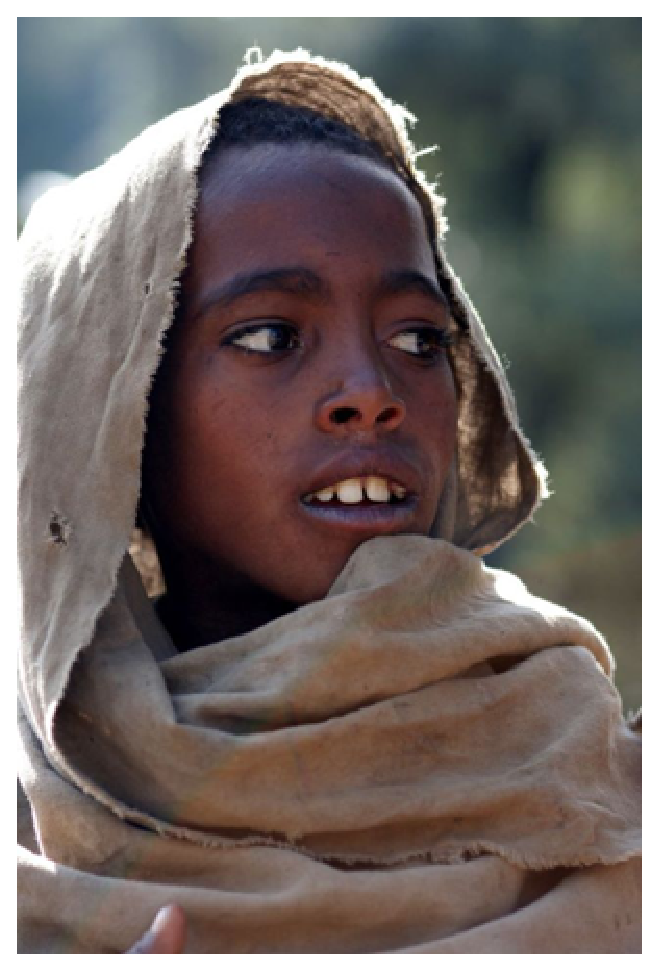
\includegraphics{etiopan.eps}}
    \reflectbox{\scalebox{0.45}{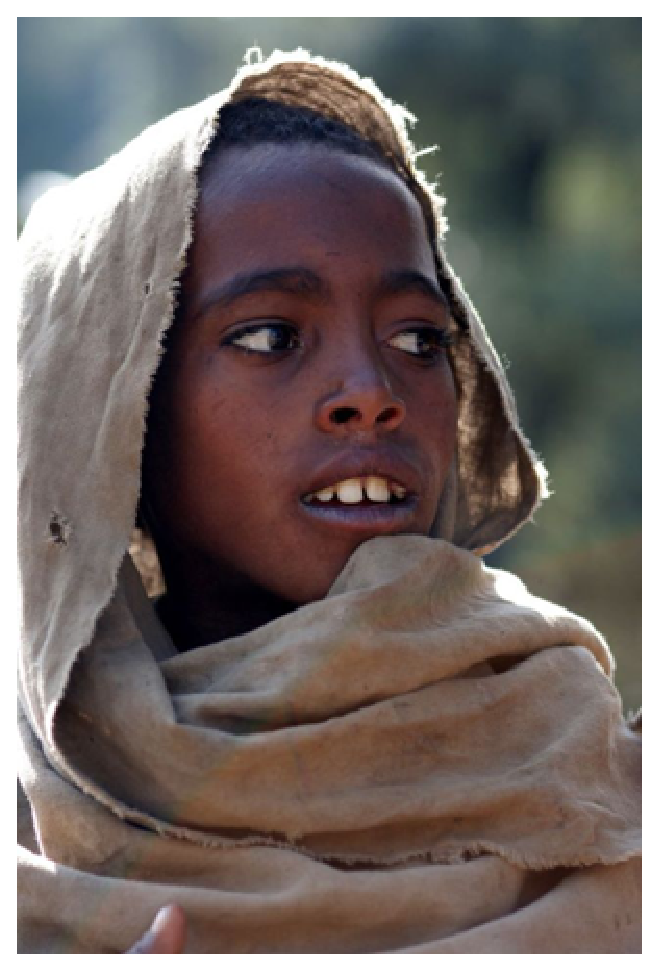
\includegraphics{etiopan.eps}}}
    \caption{Malý Etiopánek a jeho bratříček}
    \label{img:1}
\end{figure}

\newpage

Rozdíl mezi vektorovým...
\begin{figure}[h]
    \centering
    \scalebox{0.5}{
\includegraphics{oniisan.eps}}
    \caption{Vektorový obrázek}
    \label{img:2}
\end{figure}

...a bitmapovým obrázkem
\begin{figure}[h]
    \centering
    \scalebox{0.75}{
\includegraphics{oniisan2.eps}}
    \caption{Bitmapový obrázek}
    \label{img:3}
\end{figure}

se projeví například při zvětšení.

Odkazy (nejen ty) na obrázky \ref*{img:1}, \ref*{img:2} a \ref*{img:3}, na tabulky \ref*{tab:1} a \ref*{tab:2} a také na algoritmus \ref*{algo:1} jsou udělány pomocí křížových odkazů. Pak je ovšem potřeba zdrojový soubor přeložit dvakrát.

Vektorové obrázky lze vytvořit i přímo v Latexu, například pomocí prostředí \texttt{picture}.

\newpage

\begin{landscape}

\begin{figure}

\fbox{
\begin{picture}(23,10)
    
\put(20,8){\circle{2}}

\linethickness{0.1cm}
\put(1,1.5){\line(1,0){21}}


\linethickness{0.04cm}

\put(5,1.5){\line(0,1){1.5}}
\put(5,3){\line(1,0){3.5}}
\put(8.5,3){\line(3,-1){4.5}}

\put(10,2.5){\line(1,0){10.5}}
\put(20.5,2.5){\line(0,-1){1}}

\put(9,2.85){\line(0,1){1}}
\put(9,3.85){\line(1,0){11}}
\put(20,3.85){\line(0,-1){1.32}}

\put(7,3){\line(-2,3){1}}

\put(6,4.5){\line(0,1){0.7}}
\put(6,4.5){\line(1,0){14.5}}
\put(6,5.2){\line(1,0){14.5}}
\put(20.5,4.5){\line(0,1){0.7}}

\put(8,5.2){\line(0,1){1}}
\put(8,6.2){\line(1,0){6}}
\put(14,5.2){\line(0,1){1}}

\put(3.5,1.5){\line(0,1){4.2}}
\put(3.5,5.7){\line(1,0){4.5}}

\put(14,5.5){\line(1,0){5.5}}
\put(19.5,5.2){\line(0,1){0.3}}

\end{picture}
}
\caption{Vektorový obrázek moderního bydlení vhodného pro 21. století. (Buďto vytvořte stejný obrázek, anebo nakreslete pomocí \texttt{picture} váš vlastní domov.)}
\end{figure}

%TODO: add caption
\end{landscape}

\end{document}
